%%%%%%%%%%%%%%%%%%%%%%%%%%%%%%%%%%%%%%%%%%%%%%%%%%%%%%%%%%%%%%%%%%%%%%%%%%%%%%%
% CASE STUDY TEMPLATE - Programming and Problem Solving
% Author: Brendan Shea, PhD
% Course: Programming and Problem Solving
% Rochester Community and Technical College
%
% TEMPLATE INSTRUCTIONS:
% 1. Change \cstitle, \cssubtitle, \csauthor, \cscourse for each case study
% 2. Modify the main content sections as needed
% 3. Update key terms in the glossary
% 4. Adjust discussion questions for each topic
%%%%%%%%%%%%%%%%%%%%%%%%%%%%%%%%%%%%%%%%%%%%%%%%%%%%%%%%%%%%%%%%%%%%%%%%%%%%%%%

\documentclass[11pt,letterpaper]{article}

%---------- PACKAGES ----------%
\usepackage[margin=1in, headheight=22pt]{geometry}
\usepackage{xcolor}
\usepackage{tcolorbox}
\usepackage{graphicx}
\usepackage{fontspec}
\usepackage{titlesec}
\usepackage{enumitem}
\usepackage{fancyhdr}
\usepackage{listings}
\usepackage{hyperref}
\usepackage{multicol}
\usepackage{booktabs}
\usepackage{tikz}
\usepackage{float}

% TikZ libraries
\usetikzlibrary{shapes.geometric, arrows.meta, positioning, calc, backgrounds, fit}

% Load tcolorbox libraries
\tcbuselibrary{skins,breakable,listings,listingsutf8}

%---------- COLOR DEFINITIONS ----------%
% Primary palette - Magazine style
\definecolor{csprimary}{HTML}{2C3E50}      % Dark blue-gray (headers)
\definecolor{cssecondary}{HTML}{E74C3C}    % Vibrant red (accents)
\definecolor{cstertiary}{HTML}{3498DB}     % Bright blue (links, highlights)
\definecolor{csaccent}{HTML}{27AE60}       % Green (success, code)
\definecolor{cswarm}{HTML}{F39C12}         % Orange (warnings, callouts)
\definecolor{cslight}{HTML}{ECF0F1}        % Light gray (backgrounds)
\definecolor{csdark}{HTML}{1A252F}         % Very dark (code backgrounds)

% Syntax highlighting colors
\definecolor{codegreen}{HTML}{27AE60}
\definecolor{codepurple}{HTML}{9B59B6}
\definecolor{codeorange}{HTML}{E67E22}
\definecolor{codeblue}{HTML}{3498DB}
\definecolor{codegray}{HTML}{95A5A6}
\definecolor{codestring}{HTML}{E74C3C}
\definecolor{codebg}{HTML}{1E2A38}

%---------- CASE STUDY METADATA ----------%
% Modify these for each case study
\newcommand{\cstitle}{A Little History of Programming}
\newcommand{\cssubtitle}{8 Versions of Hello to \{Name\}}
\newcommand{\csauthor}{Brendan Shea, PhD}
\newcommand{\cscourse}{Programming and Problem Solving}
\newcommand{\csinstitution}{Rochester Community and Technical College}
\newcommand{\csdate}{\today}

%---------- LISTINGS CONFIGURATION ----------%
% Base style for all languages
\lstdefinestyle{basestyle}{
    backgroundcolor=\color{codebg},
    basicstyle=\ttfamily\small\color{white},
    breakatwhitespace=false,
    breaklines=true,
    captionpos=b,
    keepspaces=true,
    showspaces=false,
    showstringspaces=false,
    showtabs=false,
    tabsize=4,
    frame=none,
    xleftmargin=4mm,
    xrightmargin=4mm,
    aboveskip=0pt,
    belowskip=0pt,
}

% Assembly style
\lstdefinestyle{asmstyle}{
    style=basestyle,
    language=[x86masm]Assembler,
    keywordstyle=\color{codeblue}\bfseries,
    commentstyle=\color{codegray}\itshape,
    stringstyle=\color{codestring},
    morekeywords={section, global, db, resb, mov, syscall, rax, rdi, rsi, rdx},
}

% COBOL style
\lstdefinestyle{cobolstyle}{
    style=basestyle,
    language=COBOL,
    keywordstyle=\color{codeblue}\bfseries,
    commentstyle=\color{codegray}\itshape,
    stringstyle=\color{codestring},
    morekeywords={IDENTIFICATION, DIVISION, PROGRAM-ID, DATA, WORKING-STORAGE, SECTION, PROCEDURE, DISPLAY, ACCEPT, STOP, RUN, PIC},
}

% Fortran style
\lstdefinestyle{fortranstyle}{
    style=basestyle,
    language=Fortran,
    keywordstyle=\color{codeblue}\bfseries,
    commentstyle=\color{codegray}\itshape,
    stringstyle=\color{codestring},
    morekeywords={program, character, len, print, read, end, trim},
}

% C style
\lstdefinestyle{cstyle}{
    style=basestyle,
    language=C,
    keywordstyle=\color{codeblue}\bfseries,
    commentstyle=\color{codegray}\itshape,
    stringstyle=\color{codestring},
    morecomment=[l]{//},
}

% Java style
\lstdefinestyle{javastyle}{
    style=basestyle,
    language=Java,
    keywordstyle=\color{codeblue}\bfseries,
    commentstyle=\color{codegray}\itshape,
    stringstyle=\color{codestring},
    morekeywords={String, Scanner, System},
}

% JavaScript style
\lstdefinestyle{jsstyle}{
    style=basestyle,
    language=Java,  % Base on Java syntax
    keywordstyle=\color{codeblue}\bfseries,
    commentstyle=\color{codegray}\itshape,
    stringstyle=\color{codestring},
    morekeywords={const, let, var, function, require, console, prompt, alert},
}

% Python style
\lstdefinestyle{pythonstyle}{
    style=basestyle,
    language=Python,
    keywordstyle=\color{codeblue}\bfseries,
    commentstyle=\color{codegray}\itshape,
    stringstyle=\color{codestring},
    morekeywords={input, print, f},
}

% Plain text style (for prompts)
\lstdefinestyle{plainstyle}{
    style=basestyle,
    keywordstyle=\color{white},
    commentstyle=\color{codegray}\itshape,
}

%---------- CUSTOM ENVIRONMENTS ----------%

% Key term highlighting
\newcommand{\keyterm}[1]{\textbf{\textcolor{cssecondary}{#1}}}

% Callout box for important concepts
\newtcolorbox{conceptbox}[1][]{
    enhanced,
    colback=cslight,
    colframe=csprimary,
    fonttitle=\bfseries\color{white},
    title=#1,
    attach boxed title to top left={yshift=-2mm, xshift=5mm},
    boxed title style={colback=csprimary},
    breakable
}

% Code box using tcblisting - handles page breaks properly
% The "every listing line" option forces white color at start of each line
\newtcolorbox{codebox}[2][]{
    enhanced,
    colback=codebg,
    colframe=csaccent,
    colupper=white,
    fonttitle=\bfseries\color{white},
    title=#2,
    attach boxed title to top left={yshift=-2mm, xshift=5mm},
    boxed title style={colback=csaccent},
    left=0mm, right=0mm, top=2mm, bottom=2mm,
    boxrule=1pt,
    breakable,
    pad at break=2mm,
    before upper={\color{white}},
    #1
}

% Define tcblisting environments for each language - these handle page breaks correctly
% colupper=white ensures text color persists across page breaks
\newtcblisting{asmcode}[1][]{
    enhanced,
    colback=codebg,
    colframe=csaccent,
    colupper=white,
    colupper=white,
    fonttitle=\bfseries\color{white},
    title=#1,
    attach boxed title to top left={yshift=-2mm, xshift=5mm},
    boxed title style={colback=csaccent},
    left=0mm, right=0mm, top=2mm, bottom=2mm,
    boxrule=1pt,
    breakable,
    pad at break=2mm,
    listing only,
    listing options={style=asmstyle}
}

\newtcblisting{cobolcode}[1][]{
    enhanced,
    colback=codebg,
    colframe=csaccent,
    colupper=white,
    fonttitle=\bfseries\color{white},
    title=#1,
    attach boxed title to top left={yshift=-2mm, xshift=5mm},
    boxed title style={colback=csaccent},
    left=0mm, right=0mm, top=2mm, bottom=2mm,
    boxrule=1pt,
    breakable,
    pad at break=2mm,
    listing only,
    listing options={style=cobolstyle}
}

\newtcblisting{fortrancode}[1][]{
    enhanced,
    colback=codebg,
    colframe=csaccent,
    colupper=white,
    fonttitle=\bfseries\color{white},
    title=#1,
    attach boxed title to top left={yshift=-2mm, xshift=5mm},
    boxed title style={colback=csaccent},
    left=0mm, right=0mm, top=2mm, bottom=2mm,
    boxrule=1pt,
    breakable,
    pad at break=2mm,
    listing only,
    listing options={style=fortranstyle}
}

\newtcblisting{ccode}[1][]{
    enhanced,
    colback=codebg,
    colframe=csaccent,
    colupper=white,
    fonttitle=\bfseries\color{white},
    title=#1,
    attach boxed title to top left={yshift=-2mm, xshift=5mm},
    boxed title style={colback=csaccent},
    left=0mm, right=0mm, top=2mm, bottom=2mm,
    boxrule=1pt,
    breakable,
    pad at break=2mm,
    listing only,
    listing options={style=cstyle}
}

\newtcblisting{javacode}[1][]{
    enhanced,
    colback=codebg,
    colframe=csaccent,
    colupper=white,
    fonttitle=\bfseries\color{white},
    title=#1,
    attach boxed title to top left={yshift=-2mm, xshift=5mm},
    boxed title style={colback=csaccent},
    left=0mm, right=0mm, top=2mm, bottom=2mm,
    boxrule=1pt,
    breakable,
    pad at break=2mm,
    listing only,
    listing options={style=javastyle}
}

\newtcblisting{jscode}[1][]{
    enhanced,
    colback=codebg,
    colframe=csaccent,
    colupper=white,
    fonttitle=\bfseries\color{white},
    title=#1,
    attach boxed title to top left={yshift=-2mm, xshift=5mm},
    boxed title style={colback=csaccent},
    left=0mm, right=0mm, top=2mm, bottom=2mm,
    boxrule=1pt,
    breakable,
    pad at break=2mm,
    listing only,
    listing options={style=jsstyle}
}

\newtcblisting{pythoncode}[1][]{
    enhanced,
    colback=codebg,
    colframe=csaccent,
    colupper=white,
    fonttitle=\bfseries\color{white},
    title=#1,
    attach boxed title to top left={yshift=-2mm, xshift=5mm},
    boxed title style={colback=csaccent},
    left=0mm, right=0mm, top=2mm, bottom=2mm,
    boxrule=1pt,
    breakable,
    pad at break=2mm,
    listing only,
    listing options={style=pythonstyle}
}

\newtcblisting{plaincode}[1][]{
    enhanced,
    colback=codebg,
    colframe=csaccent,
    colupper=white,
    fonttitle=\bfseries\color{white},
    title=#1,
    attach boxed title to top left={yshift=-2mm, xshift=5mm},
    boxed title style={colback=csaccent},
    left=0mm, right=0mm, top=2mm, bottom=2mm,
    boxrule=1pt,
    breakable,
    pad at break=2mm,
    listing only,
    listing options={style=plainstyle}
}

% Discussion question box
\newtcolorbox{questionbox}{
    enhanced,
    colback=cswarm!10,
    colframe=cswarm,
    fonttitle=\bfseries\color{white},
    title=Discussion Questions,
    attach boxed title to top center={yshift=-2mm},
    boxed title style={colback=cswarm},
    breakable
}

% Timeline entry box
\newtcolorbox{timelinebox}[1][]{
    enhanced,
    colback=cstertiary!10,
    colframe=cstertiary,
    fonttitle=\bfseries,
    title=#1,
    left=2mm, right=2mm,
    boxrule=0.5pt
}

% Glossary box
\newtcolorbox{glossarybox}{
    enhanced,
    colback=cslight,
    colframe=csprimary,
    fonttitle=\bfseries\color{white},
    title=Glossary of Key Terms,
    attach boxed title to top center={yshift=-2mm},
    boxed title style={colback=csprimary},
    breakable
}

%---------- HEADER/FOOTER ----------%
\pagestyle{fancy}
\fancyhf{}
\fancyhead[L]{\small\textcolor{csprimary}{\cscourse}}
\fancyhead[R]{\small\textcolor{csprimary}{Case Study}}
\fancyfoot[C]{\thepage}
\renewcommand{\headrulewidth}{0.4pt}
\renewcommand{\headrule}{\hbox to\headwidth{\color{csprimary}\leaders\hrule height \headrulewidth\hfill}}

%---------- SECTION FORMATTING ----------%
\titleformat{\section}
    {\Large\bfseries\color{csprimary}}
    {\thesection}{1em}{}[\color{cssecondary}\titlerule]
    
\titleformat{\subsection}
    {\large\bfseries\color{cstertiary}}
    {\thesubsection}{1em}{}

%---------- HYPERLINK SETTINGS ----------%
\hypersetup{
    colorlinks=true,
    linkcolor=cstertiary,
    urlcolor=cstertiary
}

%%%%%%%%%%%%%%%%%%%%%%%%%%%%%%%%%%%%%%%%%%%%%%%%%%%%%%%%%%%%%%%%%%%%%%%%%%%%%%%
% DOCUMENT BEGINS
%%%%%%%%%%%%%%%%%%%%%%%%%%%%%%%%%%%%%%%%%%%%%%%%%%%%%%%%%%%%%%%%%%%%%%%%%%%%%%%

\begin{document}

%---------- TITLE BLOCK ----------%
\begin{tcolorbox}[
    enhanced,
    colback=csprimary,
    colframe=csprimary,
    arc=0mm,
    left=10mm, right=10mm, top=8mm, bottom=8mm
]
\begin{center}
    {\huge\bfseries\color{white}\cstitle}\\[3mm]
    {\Large\color{cslight}\cssubtitle}\\[5mm]
    \textcolor{cssecondary}{\rule{0.5\textwidth}{1pt}}\\[5mm]
    {\large\color{white}\csauthor}\\[2mm]
    {\normalsize\color{cslight}\cscourse\ $\bullet$ \csinstitution}
\end{center}
\end{tcolorbox}

\vspace{5mm}

%---------- INTRODUCTION ----------%
\section*{Introduction}

Every programmer remembers their first program. For millions of us, that program displayed a simple greeting: ``Hello, World!'' But have you ever wondered how that simple act of saying hello has changed over nearly 80 years of computing history? In this case study, we'll explore the evolution of programming languages by examining how eight different languages---spanning from the 1950s to today---accomplish the seemingly simple task of greeting a user by name.

This journey will take us from the raw metal of \keyterm{machine code} through the revolutionary abstraction of \keyterm{high-level languages}, and finally to the frontier of \keyterm{natural language programming} with large language models. Along the way, you'll discover how each generation of programming tools reflects the technology, priorities, and philosophy of its era.

\begin{conceptbox}[The Challenge]
Write a program that asks the user for their name and then displays: ``Hello, [Name]!''

This simple task requires: getting input from a user, storing data in memory, combining text (string concatenation), and displaying output. How we accomplish these tasks reveals everything about a programming language's design philosophy.
\end{conceptbox}

%---------- TIMELINE DIAGRAM ----------%
\vspace{3mm}
\begin{center}
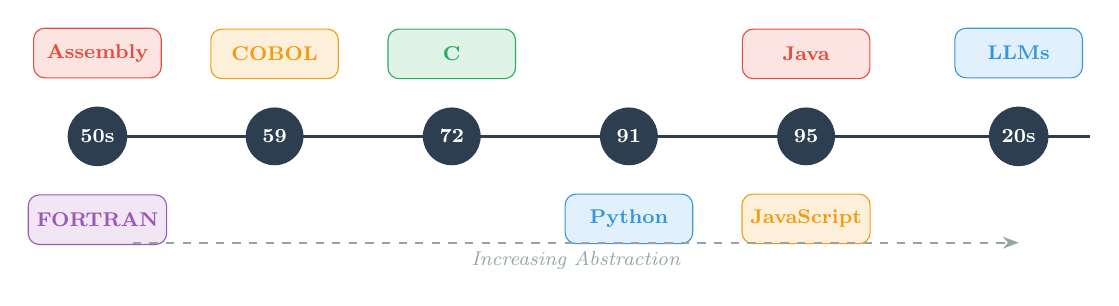
\begin{tikzpicture}[
    scale=0.9,
    transform shape,
    yearnode/.style={circle, draw=csprimary, fill=csprimary, text=white, minimum size=8mm, font=\footnotesize\bfseries},
    langnode/.style={rectangle, rounded corners, draw=#1, fill=#1!15, minimum width=18mm, minimum height=7mm, font=\footnotesize\bfseries, text=#1},
    arrow/.style={-{Stealth[length=2mm]}, thick, color=codegray}
]

% Timeline base line
\draw[very thick, color=csprimary] (0,0) -- (14,0);

% Year markers and language boxes
\node[yearnode] (y1) at (0,0) {50s};
\node[langnode=cssecondary, above=4mm of y1] (asm) {Assembly};
\node[langnode=codepurple, below=4mm of y1] (fortran) {FORTRAN};

\node[yearnode] (y2) at (2.5,0) {59};
\node[langnode=cswarm, above=4mm of y2] (cobol) {COBOL};

\node[yearnode] (y3) at (5,0) {72};
\node[langnode=csaccent, above=4mm of y3] (c) {C};

\node[yearnode] (y4) at (7.5,0) {91};
\node[langnode=codeblue, below=4mm of y4] (python) {Python};

\node[yearnode] (y5) at (10,0) {95};
\node[langnode=codestring, above=4mm of y5] (java) {Java};
\node[langnode=cswarm, below=4mm of y5] (js) {JavaScript};

\node[yearnode] (y6) at (13,0) {20s};
\node[langnode=cstertiary, above=4mm of y6] (llm) {LLMs};

% Trend arrow
\draw[arrow, dashed] (0.5,-1.5) -- (13,-1.5) node[midway, below, font=\footnotesize\itshape, text=codegray] {Increasing Abstraction};

\end{tikzpicture}
\end{center}
\vspace{2mm}

%---------- MAIN CONTENT ----------%
\section{The Pioneers: Assembly Language (1950s)}

In the earliest days of computing, programmers communicated with machines using \keyterm{assembly language}---a thin layer of human-readable mnemonics sitting directly atop the CPU's binary instructions. Each line of assembly corresponds almost one-to-one with a machine instruction. There is no hiding the computer's architecture here; you must understand registers, memory addresses, and the specific instruction set of your processor.

\begin{asmcode}[x86-64 Assembly (Linux)]
section .data                    ; Data we define ahead of time
    prompt db "Enter your name: ", 0
    hello db "Hello, ", 0
section .bss                     ; Reserve space for user input
    name resb 64                 ; 64 bytes for the name
section .text
    global _start
_start:
    ; STEP 1: Print the prompt to screen
    mov rax, 1          ; System call number for "write"
    mov rdi, 1          ; File descriptor 1 = standard output
    mov rsi, prompt     ; Address of our prompt string
    mov rdx, 17         ; Number of bytes to write
    syscall             ; Ask the operating system to do it
    
    ; STEP 2: Read the user's input
    mov rax, 0          ; System call number for "read"
    mov rdi, 0          ; File descriptor 0 = standard input  
    mov rsi, name       ; Where to store the input
    mov rdx, 64         ; Maximum bytes to read
    syscall
    
    ; STEP 3: Print "Hello, " then the name...
    ; (Additional code continues similarly)
\end{asmcode}

Notice how every operation requires explicit instructions: we must tell the CPU exactly which \keyterm{register} to use, specify memory addresses, count bytes manually, and invoke operating system services through numbered ``syscalls.'' The command \texttt{mov rax, 1} doesn't mean ``print''---it loads the number 1 into a register, which \textit{happens} to be the code for the write operation. This granular control yields maximum performance but minimal productivity.

\section{Business Computing: COBOL (1959)}

While scientists worked with numbers, the business world needed to process text, records, and reports. \keyterm{COBOL} (Common Business-Oriented Language) was designed by a committee including the legendary Grace Hopper, who believed programs should be readable like English prose.

\begin{cobolcode}[COBOL]
IDENTIFICATION DIVISION.
PROGRAM-ID. HELLO-NAME.

DATA DIVISION.
WORKING-STORAGE SECTION.
01 USER-NAME PIC X(30).         *> Reserve 30 characters for name

PROCEDURE DIVISION.
    DISPLAY "Enter your name: ".  *> Show prompt on screen
    ACCEPT USER-NAME.             *> Wait for and store input
    DISPLAY "Hello, " USER-NAME "!".  *> Combine and display
    STOP RUN.
\end{cobolcode}

The contrast with assembly is striking. COBOL reads almost like a business memo: \texttt{DISPLAY} shows text, \texttt{ACCEPT} gets input, and \texttt{PIC X(30)} declares a ``picture'' of 30 characters. The verbose DIVISIONS and SECTIONS may seem excessive, but they made programs easier to read and audit---crucial for financial applications. Remarkably, COBOL remains in use today; billions of lines still process banking transactions and government records.

\section{Scientific Roots: FORTRAN (1957)}

\keyterm{FORTRAN} (Formula Translation) holds the distinction of being the first widely adopted high-level language. Created at IBM by John Backus and his team, FORTRAN allowed scientists and engineers to write mathematical formulas in near-natural notation, with the \keyterm{compiler} translating these into efficient machine code.

\begin{fortrancode}[Fortran 90]
program hello_name
    character(len=50) :: name    ! Declare a 50-character variable
    
    print *, "Enter your name: " ! Print prompt (* means default format)
    read *, name                 ! Read input into 'name' variable
    print *, "Hello, ", trim(name), "!"  ! trim() removes extra spaces
end program hello_name
\end{fortrancode}

FORTRAN demonstrated a revolutionary concept: you could write code at a higher level of \keyterm{abstraction} and trust the compiler to produce efficient results. The \texttt{print} and \texttt{read} statements handle all the complex details of I/O that assembly required us to manage manually. The \texttt{trim()} function shows another advantage: built-in utilities that would require dozens of assembly instructions.

\section{Systems Programming: C (1972)}

Dennis Ritchie created \keyterm{C} at Bell Labs to rewrite the Unix operating system. C occupies a unique middle ground: it provides high-level conveniences like functions and structured data types while still allowing direct memory manipulation through \keyterm{pointers}.

\begin{ccode}[C]
#include <stdio.h>    // Include standard input/output library

int main() {
    char name[50];    // Create array of 50 characters for the name
    
    printf("Enter your name: ");  // Print prompt (no newline)
    scanf("%49s", name);   // Read up to 49 chars into 'name'
                           // %s = string format, 49 = safety limit
    printf("Hello, %s!\n", name);  // %s gets replaced by 'name'
    return 0;              // Return 0 = program succeeded
}
\end{ccode}

The \texttt{char name[50]} declaration reveals C's philosophy: you explicitly manage memory by declaring arrays of specific sizes. The \texttt{\%s} is a ``format specifier'' that tells \texttt{printf} where to insert the string. C's influence is immense---your operating system, web browser, and smartphone are largely written in C or its descendants. The syntax with curly braces, semicolons, and \texttt{main()} became the template for Java, JavaScript, and many others.

\section{Object-Oriented Revolution: Java (1995)}

James Gosling and his team at Sun Microsystems designed \keyterm{Java} with a bold promise: ``Write Once, Run Anywhere.'' Java programs run on a \keyterm{virtual machine} (JVM) rather than directly on hardware, enabling the same code to execute on any platform.

\begin{javacode}[Java]
import java.util.Scanner;  // Import the Scanner tool for input

public class HelloName {
    public static void main(String[] args) {
        // Create a Scanner object to read from keyboard
        Scanner scanner = new Scanner(System.in);
        
        System.out.print("Enter your name: ");  // print = no newline
        String name = scanner.nextLine();  // Read entire line of input
        
        // Concatenate strings with + operator
        System.out.println("Hello, " + name + "!");  // println = newline
        scanner.close();  // Clean up the Scanner resource
    }
}
\end{javacode}

Java introduced millions of developers to \keyterm{object-oriented programming} (OOP). Notice how we create a \texttt{Scanner} \textit{object} and call its \texttt{nextLine()} method. Everything in Java lives inside a \textit{class} (here, \texttt{HelloName}). The verbose declaration \texttt{public static void main(String[] args)} is Java's required entry point---every application starts here. This explicitness enables large teams to collaborate on massive codebases with confidence.

\section{The Web's Language: JavaScript (1995)}

Brendan Eich famously created \keyterm{JavaScript} in just ten days at Netscape. Despite its name (a marketing decision), JavaScript is completely different from Java. It brought programming directly into web browsers.

\begin{jscode}[JavaScript (Browser)]
// In a browser, these built-in functions handle everything!
const name = prompt("Enter your name:");  // Pop-up input box
alert(`Hello, ${name}!`);  // Pop-up message box
// The backticks and ${} let us embed variables in strings
\end{jscode}

\begin{jscode}[JavaScript (Node.js - Server)]
const readline = require('readline');  // Import I/O module
const rl = readline.createInterface({
    input: process.stdin,    // Read from keyboard
    output: process.stdout   // Write to screen
});

// question() displays prompt, then runs callback with answer
rl.question("Enter your name: ", (name) => {
    console.log(`Hello, ${name}!`);  // Template literal syntax
    rl.close();
});
\end{jscode}

JavaScript exemplifies \keyterm{dynamic typing}---variables like \texttt{name} don't have declared types; they can hold any kind of data. The browser version accomplishes our task in just two lines! The template literal syntax (\texttt{\`{}Hello, \$\{name\}!\`{}}) with backticks is modern JavaScript's elegant way to embed variables in strings.

\section{Readability First: Python (1991)}

Guido van Rossum created \keyterm{Python} with an explicit philosophy: code readability counts. Python's clean syntax eliminates much of the ceremony found in other languages.

\begin{pythoncode}[Python]
# Get input - input() displays prompt and returns what user types
name = input("Enter your name: ")

# Print with f-string: f"..." lets us embed {variables} directly
print(f"Hello, {name}!")
\end{pythoncode}

Two lines. No imports for basic I/O, no type declarations, no semicolons, no braces. The \texttt{f} before the string creates a ``formatted string literal'' (f-string)---Python's elegant solution for combining text and variables. Python's \keyterm{interpreted} nature means you can run code immediately without a separate compilation step. This immediacy has made Python the dominant language in data science, AI, and education.

\section{The New Frontier: Natural Language and LLMs (2020s)}

We now stand at another inflection point. \keyterm{Large Language Models} (LLMs) like GPT and Claude can generate working code from plain English descriptions:

\begin{plaincode}[Prompting an LLM]
Write a Python program that asks for the user's name 
and then greets them by saying "Hello" followed by 
their name and an exclamation point.
\end{plaincode}

This represents \keyterm{natural language programming}---describing what you want rather than how to do it. The LLM translates your intent into working code. While this technology is new and imperfect (it can produce buggy or insecure code), it suggests a future where the barrier between human intention and computer execution continues to shrink.

%---------- ABSTRACTION DIAGRAM ----------%
\section{Patterns Across Time}

\begin{center}
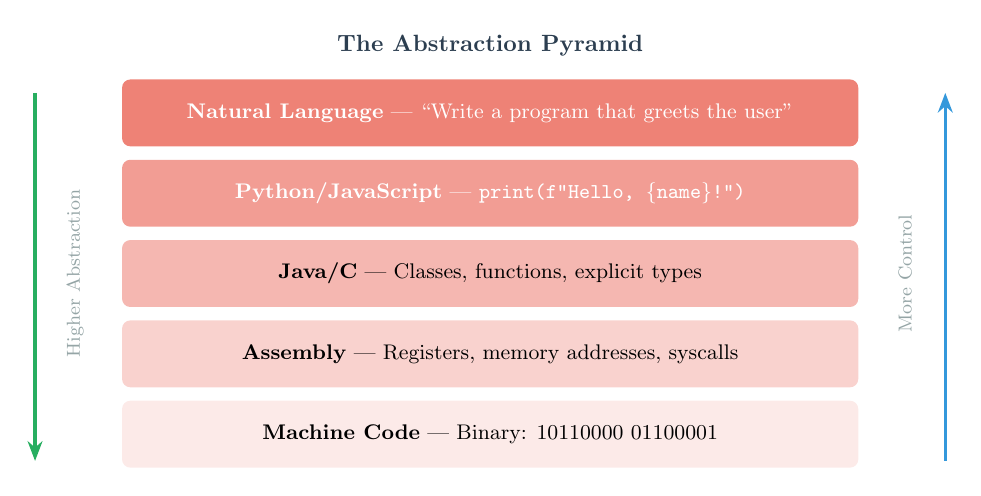
\begin{tikzpicture}[
    scale=0.85,
    transform shape,
    layer/.style={rectangle, rounded corners=3pt, minimum width=11cm, minimum height=10mm, font=\small},
    label/.style={font=\footnotesize, text=codegray},
    arrow/.style={-{Stealth[length=2.5mm]}, very thick}
]

% Background gradient effect using layers
\node[layer, fill=cssecondary!70, text=white] (l1) at (0,0) {\textbf{Natural Language} --- ``Write a program that greets the user''};
\node[layer, fill=cssecondary!55, text=white] (l2) at (0,-1.2) {\textbf{Python/JavaScript} --- \texttt{print(f"Hello, \{name\}!")}};
\node[layer, fill=cssecondary!40] (l3) at (0,-2.4) {\textbf{Java/C} --- Classes, functions, explicit types};
\node[layer, fill=cssecondary!25] (l4) at (0,-3.6) {\textbf{Assembly} --- Registers, memory addresses, syscalls};
\node[layer, fill=cssecondary!12] (l5) at (0,-4.8) {\textbf{Machine Code} --- Binary: 10110000 01100001};

% Side labels
\node[label, rotate=90] at (-6.2,-2.4) {Higher Abstraction};
\node[label, rotate=90] at (6.2,-2.4) {More Control};

% Arrows
\draw[arrow, color=csaccent] (-6.8,0.3) -- (-6.8,-5.2);
\draw[arrow, color=cstertiary] (6.8,-5.2) -- (6.8,0.3);

% Title
\node[font=\bfseries\color{csprimary}] at (0,1) {The Abstraction Pyramid};

\end{tikzpicture}
\end{center}

\vspace{2mm}

Looking at these eight approaches, several patterns emerge. First, there is a clear trend toward \textbf{higher abstraction}---each generation hides more complexity, allowing programmers to think about \textit{what} they want rather than \textit{how} the machine accomplishes it. Second, we see increasing emphasis on \textbf{readability}. From COBOL's English-like syntax to Python's clean design, language creators recognize that code is read far more often than it is written. Third, the \textbf{target audience} has expanded dramatically. Early languages served specialists with deep hardware knowledge; modern languages welcome beginners. Finally, the very definition of ``programming'' is shifting---from manipulating registers to describing intentions in natural language.

Yet older languages persist. COBOL processes trillions in transactions. FORTRAN dominates scientific supercomputing. C underlies virtually every operating system. Each language found its niche and, once embedded in critical systems, proved remarkably durable. The best language is always the one that fits the problem, the team, and the context.

%---------- DISCUSSION QUESTIONS ----------%
\section*{Discussion Questions}

\begin{questionbox}
\begin{enumerate}[leftmargin=*, label=\textcolor{cswarm}{\textbf{\arabic*.}}]
    \item \textbf{Trade-offs in Abstraction:} Assembly language gives programmers complete control but requires extensive expertise. Python hides many details but limits control over performance. When might the trade-off favor lower-level languages? Consider embedded systems, game engines, operating systems, web applications, and data analysis scripts.
    
    \item \textbf{The COBOL Paradox:} COBOL is often mocked as outdated, yet it processes trillions of dollars in transactions daily and there's a shortage of COBOL programmers. Why do organizations continue using 60-year-old technology? What does this tell us about the relationship between programming languages and the systems that depend on them?
    
    \item \textbf{Natural Language Programming:} If LLMs can generate code from English descriptions, what skills will programmers need in the future? Will ``prompt engineering'' replace traditional coding, or will understanding programming fundamentals remain essential for debugging, security, and system design?
    
    \item \textbf{Design Philosophy:} Java emphasizes explicit type declarations and verbose syntax; Python emphasizes brevity and readability. Both have passionate advocates. How might team size, project lifespan, or application domain (finance vs. startups vs. scientific research) affect which philosophy is preferable?
    
    \item \textbf{Historical Contingency:} JavaScript was created in ten days and now runs on billions of devices. Some languages with elegant designs (like Lisp or Haskell) remain niche. How much of a programming language's success comes from technical merit versus historical accident, corporate backing, or simply being available at the right moment?
\end{enumerate}
\end{questionbox}

%---------- GLOSSARY ----------%
\section*{Key Terms}

\begin{glossarybox}
\begin{description}[leftmargin=!, labelwidth=3.5cm, font=\bfseries\color{cssecondary}]
    \item[Abstraction] Hiding complex implementation details behind simpler interfaces, allowing programmers to work at higher conceptual levels without managing every detail.
    
    \item[Assembly Language] A low-level language using mnemonic codes (like MOV, ADD) that correspond directly to a processor's machine instructions.
    
    \item[COBOL] Common Business-Oriented Language (1959); designed for business data processing with English-like, self-documenting syntax.
    
    \item[Compiler] A program that translates human-readable source code into machine code before the program runs, enabling optimization and error checking.
    
    \item[Dynamic Typing] A language feature where variable types are determined at runtime rather than declared in advance, offering flexibility but fewer compile-time checks.
    
    \item[FORTRAN] Formula Translation (1957); the first widely-used high-level language, designed for scientific and mathematical computing.
    
    \item[High-Level Language] A programming language that abstracts away hardware details, allowing portable, human-readable code.
    
    \item[Interpreted] Executing code line-by-line through an interpreter rather than compiling it to machine code first, enabling immediate feedback.
    
    \item[Large Language Model] An AI system trained on vast text data that can generate human-like text and code from natural language prompts.
    
    \item[Machine Code] Binary instructions (1s and 0s) that a CPU executes directly---the lowest level of software.
    
    \item[Natural Language Programming] Using human language to instruct computers, often via AI systems that translate intent into executable code.
    
    \item[Object-Oriented Programming] A paradigm organizing code into ``objects'' containing both data and the methods that operate on that data.
    
    \item[Pointer] A variable storing a memory address, enabling direct memory manipulation---powerful but error-prone.
    
    \item[Register] A small, ultra-fast storage location inside a CPU, used for data being actively processed.
    
    \item[Virtual Machine] A software layer executing code independently of underlying hardware, enabling platform-independent programs (e.g., Java's JVM).
\end{description}
\end{glossarybox}

\vspace{5mm}

%---------- FOOTER ----------%
\begin{center}
\textcolor{csprimary}{\rule{0.6\textwidth}{0.5pt}}\\[3mm]
{\small\textcolor{gray}{This case study is part of the Open Educational Resources for \cscourse.\\
Licensed under Creative Commons Attribution 4.0 (CC BY 4.0).}}
\end{center}

\end{document}